
\RequirePackage{fix-cm}
%
\RequirePackage{amsmath}

%\documentclass{svjour3}                     % onecolumn (standard format)
%\documentclass[smallcondensed]{svjour3}     % onecolumn (ditto)
%\documentclass[smallextended]{svjour3}       % onecolumn (second format)
\documentclass[twocolumn]{svjour3}          % twocolumn
%\documentclass[letterpaper, 12pt, twocolumn]{article}

%\usepackage[margin=1in]{geometry}
\usepackage{amssymb}
\usepackage{graphicx}
\usepackage[utf8]{inputenc}
\usepackage{indentfirst}
\usepackage{physics}
\newcommand{\me}{\mathrm{e}}
\usepackage{amsmath}

%\usepackage[round]{natbib}
%\usepackage{apacite}
\usepackage{url} % not crucial - just used below for the URL 

%\providecommand{\keywords}[1]{\textbf{\textit{Index terms---}} #1}

\begin{document}



\title{Algorithm to generate multi-factorial experiments to teach experimental design%\thanks{Grants or other notes
%about the article that should go on the front page should be
%placed here. General acknowledgments should be placed at the end of the article.}
}
\subtitle{Do you have a subtitle?\\ If so, write it here}
%\titlerunning{Short form of title}        % if too long for running head
\author{Cristy  \and
        Nagamani \and
        Raji \and
        S. K. Gadi
}
%\authorrunning{Short form of author list} % if too long for running head
\institute{     Cristy \at
                first address
            \and
                Nagamani \at
                first address
           \and
                Raji \at
                second address
            \and
                S. K. Gadi \at
                FIME, Universidad Autónoma de Coahuila,  Torreón, México\\
                Tel.: (+52 1) 871-757-0153\\
                Fax: (+52 1) 871 757 0153\\
                \email{research@skgadi.com}
}
\date{Received: date / Accepted: date}
% The correct dates will be entered by the editor
\maketitle
\begin{abstract}
One of the challenges in teaching the subject, Design of Experiments, is to come up with a proper numerical example. In this article, authors present a methodology to generate a numerical example for multifactorial experiments. Also, it presents a simple algorithm, which can be implemented in any programming language to generate unique examples.
\end{abstract}
\keywords{Experimental design; educational tool; generating examples}
\section{Introduction}
Experimental design is applied in almost all the fields involving experimentation \cite{fisher1937design,quinn2002experimental,montgomery2008design,antony2014design}. It is part of various undergraduate and graduate curriculum, ranging from the engineering to the biological sciences. In general the objective of experimental design is to minimize cost and time of the experiments and maximize the yield. Improper design of experiment may lead to inaccurate or false conclusions, as well as a loss of money, material and time \cite{Festing2003341}.
\par
Learning statistics or mathematics in general is effective by solving a number of numerical examples \cite{zhu1987learning}. It helps the students to develop insight in the topics \cite{renkl1997learning}. Teachers may involve students in finding experiments to teach the topic \cite{Hunter1977Some,fried2006mathematics,Hiebert82}. However, it is teacher's task to generate examples for the classroom and for the practise \cite{Deborah2008}.
\par
Solving optimization problems, finding mathematical model etc. in experimental design involves performing various experiments with a different combinations of the factors. Conducting experiments on a real system for the classroom purpose is not always feasible due to any the following limitations.
\begin{enumerate}
	\item The cost of conducting experiments on a real system is not always negligible.
	\item A considerable amount of time may take for each experiment.
	\item The combination of factors associated for optimum response is constant for a physical system. Therefore, teachers may not provide a fresh problem.
\end{enumerate}
\par
Hence, a computer program generating responses for the given input factors is a good alternative to mimic the physical systems. In this article we present a methodology to generate numerical examples which simulate experiments. The objective is to generate unique process for the limits selected by the user, which ouputs experimental data for the given combinations of the factors. Teachers may adopt this methodology in generating numerical examples, which highlight all the characteristics they want to present to the classroom, give as practice exercise and conduct exams.
\par
The proposed algorithm is described in Section \ref{Sec:Algorithm}. Readers interested only in the implementation of algorithm may skip the mathematical construction presented in Section \ref{Sec:Construction} and \ref{Sec:Adapting}.
\par
A numerical example for an experimental design is a mathematical model representing a physical process. This model is a set of static functions (i.e. it does not have derivative or integral terms) which maps the factors to the responses. A real life system may present more than one peaks. However, most of the experimental design methods find the local maximum based on the initial base value. Hence, the proposed algorithm is designed to present only one peak. A multi-response system can be represented as %Because time is also a factor
\begin{eqnarray}
y_j &=& f_j(x_1, x_2, x_3, \dots, x_n) + \xi_j \label{Eqn:Function}
\end{eqnarray}
\noindent where $y_j$, $j\in \{1,2,3, \dots, m\}$ are the responses, $x_i$, $i\in \{1,2,3, \dots, n\}$ are the factors, $f_j$, $j\in \{1,2,3, \dots, m\}$ are the nonlinear functions mapping the $n$ factors to the $m$ responses and $\xi_i$, $i\in \{1,2,3, \dots, m\}$ are the noise.
\par
All the factors, $x_i$, are constrained by upper and lower limits. The numerical examples should produce an unique optimal responses, $y_j^M$, for a set of factors within its limits. Construction of a one such mathematical function is presented in the next section.
\par
The proposed algorithm presents the case of single response, which can be adopted to multi-response.
\section{Construction of a mathematical function to suit our requirements}
\label{Sec:Construction}
\subsection{Quadratic concave function}
\begin{figure}
	\centering
	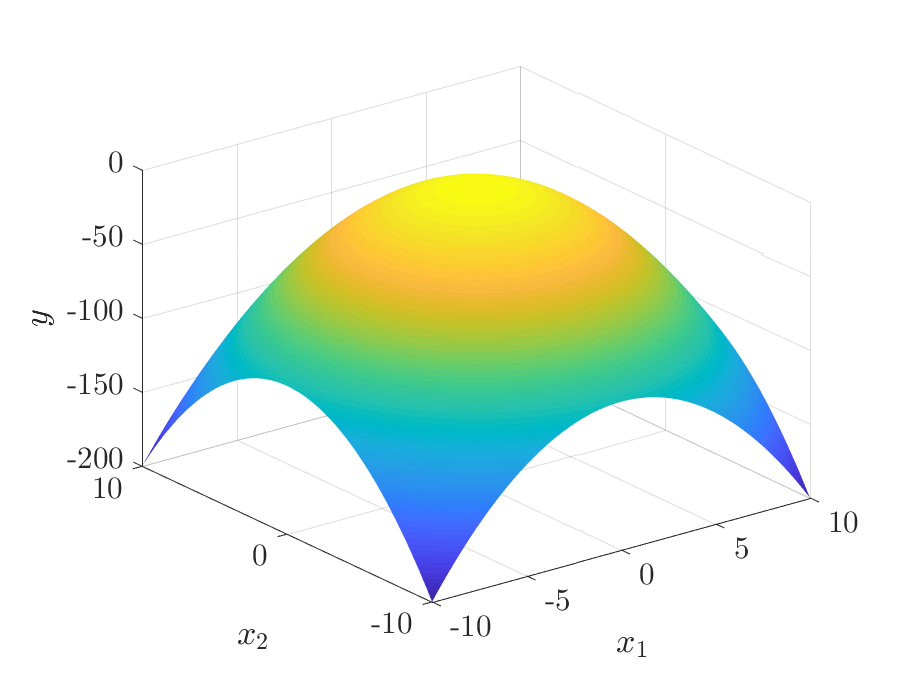
\includegraphics[width=0.48\textwidth]{images/poly-2-var}
	\label{Fig:TwoVariablePolynomial}
	\caption{A second order polynomial convex function}
\end{figure}
A second order polynomial function, such as
\begin{eqnarray}
F(x_1, x_2, x_3, \dots, x_n) &=& -\sum_{i=1}^{n}{x_i^2} \label{Eqn:PolyFunction}
\end{eqnarray}
is a concave function, which serve the purpose of providing a unique optimal point. Figure~\ref{Fig:TwoVariablePolynomial} depicts (\ref{Eqn:PolyFunction}) for the two variables case. However, it doesn't meet the requirements of a good example because to the following limitations.
\begin{enumerate}
	\item Response surface methodology uses a second order fit algorithm. Hence, the process of reaching optimal solution becomes trivial.
	\item A quadratic function is having a property that its slope increases as it moves far from the optimal point. This property trivializes the process of selecting a new base value.
\end{enumerate}
\subsection{Multivariable Gaussian function}
\begin{figure}
	\centering
	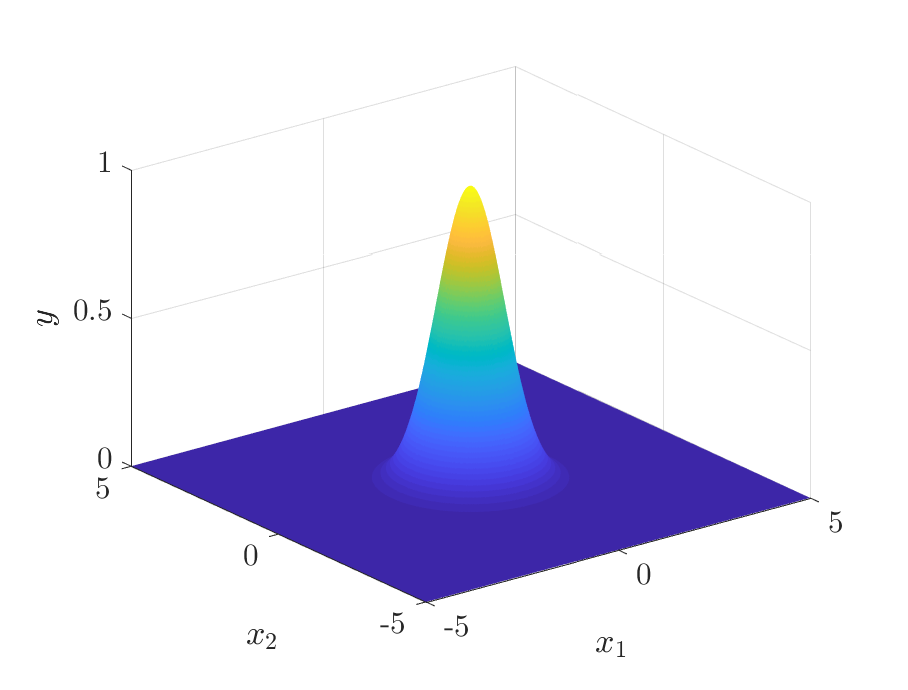
\includegraphics[width=0.48\textwidth]{images/2GussianFunction}
	\label{Fig:TwoVarGaussian}
	\caption{Two variable Gaussian distribution function}
\end{figure}
The multivariable Gussian function
\begin{eqnarray}
	F(x_1, x_2, x_3, \dots, x_n) = \prod_{i=1}^{n}{\me^{-x_i^2}} \label{Eqn:MultiFactorialNormal}
\end{eqnarray}
is a concave function, hence, it has a unique maximum value. The slope of this function is not linearly related with the distance from its optimal point. The concave functions have property that the response of all the points between any two arbitrary points always grater than the responses at these arbitrary points \cite{antoniou2007practical}. A non-concave function gives additional challenge in solving the optimization problem. 
\subsection{Sigmoid convex function}
\begin{figure}
	\centering
	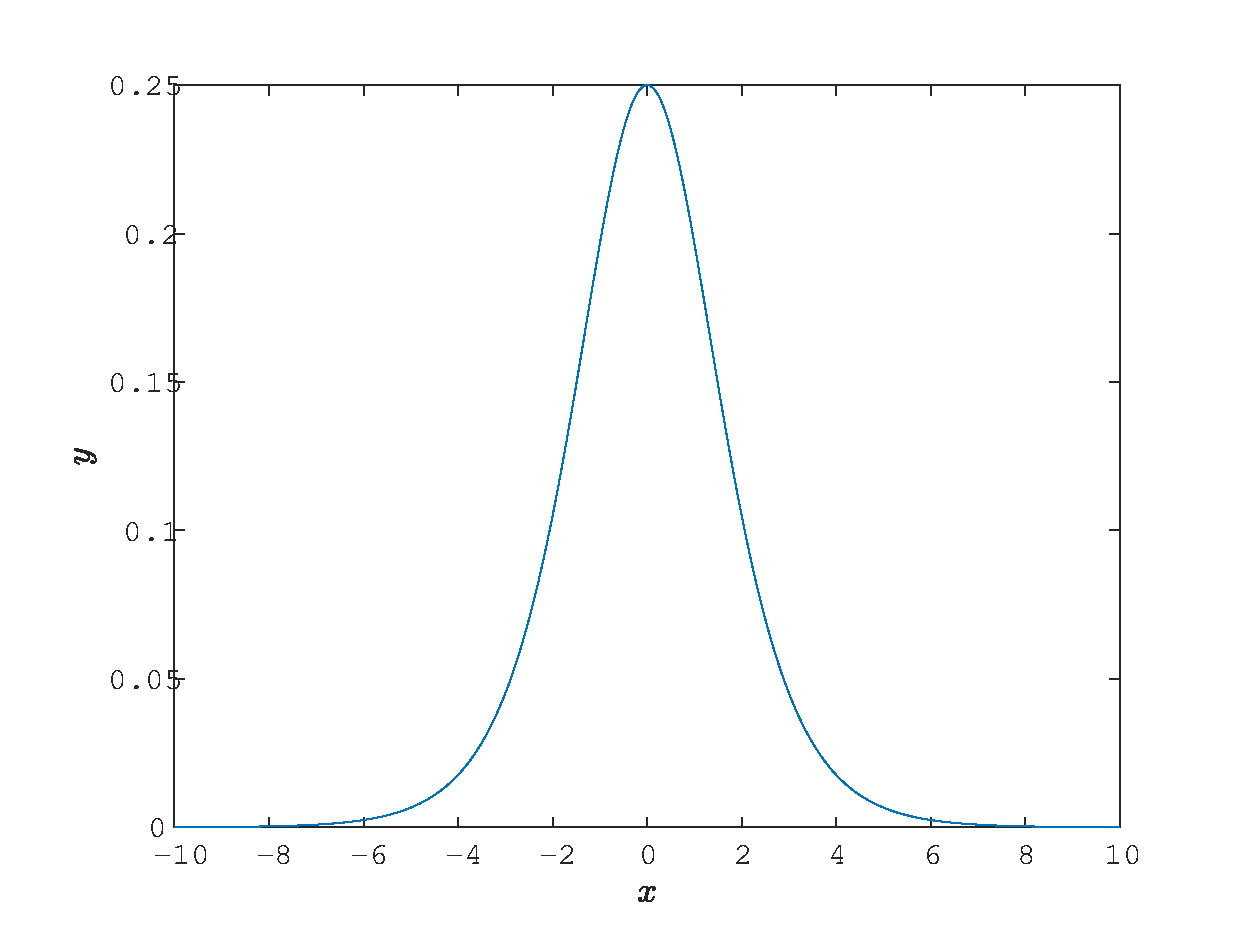
\includegraphics[width=0.48\textwidth]{images/1FactorsSigmoid}
	\label{Fig:OneVarSigmoid}
	\caption{One variable convex function}
\end{figure}
\begin{figure}
	\centering
	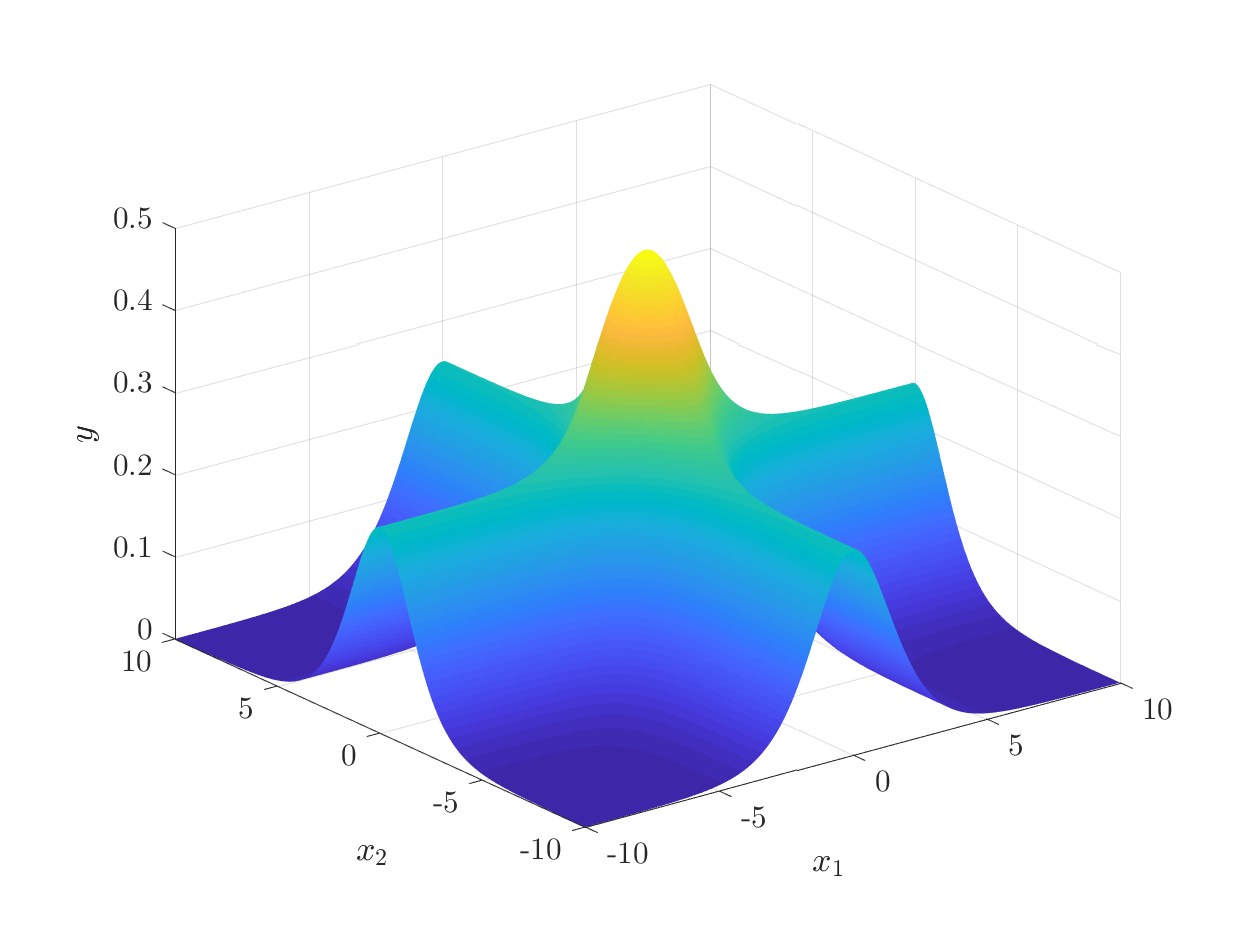
\includegraphics[width=0.48\textwidth]{images/2FactorsSigmoid}
	\label{Fig:MultiVarSigmoid}
	\caption{Two variable convex function}
\end{figure}
Keeping above limitations in mind, a sigmoid based convex function is proposed. One variable sigmoid function is
\begin{eqnarray}
S(x) = \frac{1}{1-\me^{-x}} \label{Eqn:Sigmoid}
\end{eqnarray}
and its derivative is
\begin{eqnarray}
F(x) = S'(x) = \frac{\me^x}{(\me^{x}+1)^2} = S(x)(1-S(x)). \label{Eqn:DiffSigmoid}
\end{eqnarray}
\par
The function $F$ is plotted in Figure~\ref{Fig:OneVarSigmoid}. The function $F$ can be extended to a $n$ variables case as
\begin{eqnarray}
F(x_1, x_2, x_3, ..., x_n) = \sum_{i=1}^{n}{\frac{\me^x_i}{(\me^{x_i}+1)^2}}. \label{Eqn:DiffSigmoidMulti}
\end{eqnarray}
\par
Figure~\ref{Fig:MultiVarSigmoid} shows sigmoid based function for two variables. A function can be said concave, if Hessian matrix associated with it is negative definite \cite{bernstein1962some}. Hessian matrix for (\ref{Eqn:DiffSigmoidMulti}) is 
\begin{eqnarray}
H_{i,j} = \pdv[2]{F}{x_i} =
\begin{cases}
\frac{\me^{x_i}(\me^{2x_i}-4\me^{x_i}+1)}{(\me^{x_i}+1)^2},& \text{if } i = j\\
0,              & \text{otherwise.}
\end{cases} \label{Eqn:HessianMatrix}
\end{eqnarray}
\par
It can be observed that the Hessian matrix, $H_{i,j}$, is not a negative definite because this diagonal matrix is positive definite for $x_i<\ln({2-\sqrt{3}})$ and $x_i<\ln({2+\sqrt{3}})$.
\par
The Hessian matrix, $H_{i,j}$ is having a not a negative definite because it is a diagonal matrix and the diagnal values are positive. Hence, $F$ is a convex function, i.e. has a unique maximum value with no other peaks. In the next section a method is presented to adapt $F$ to generate random experiments within given limits.
\par
Not using normal distribution because we can tune this further to get a non-symmetric equation.
\begin{figure}
	\centering
	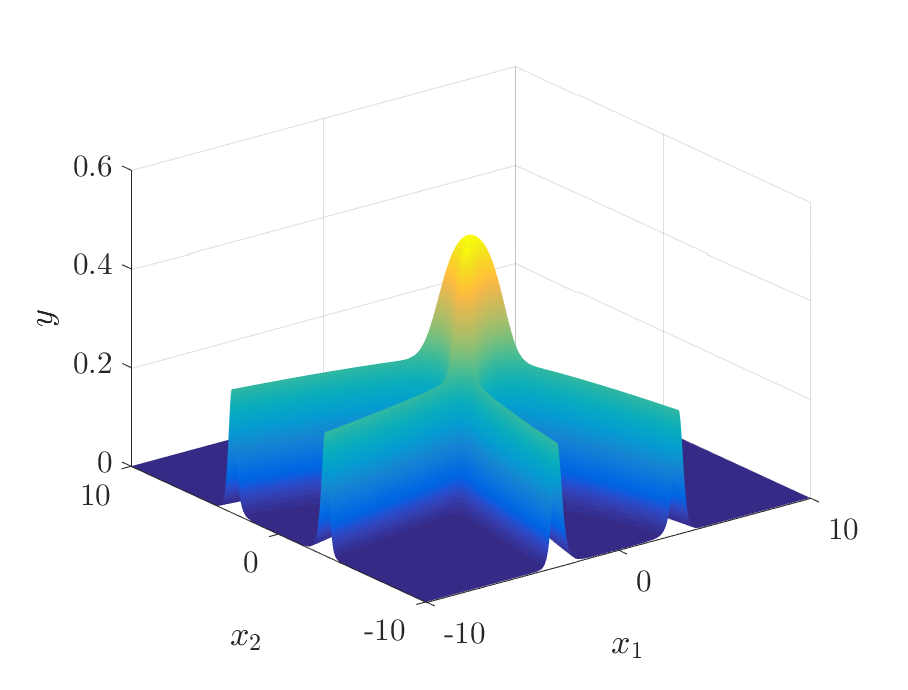
\includegraphics[width=0.48\textwidth]{images/2FactorsSigmoidFuture}
	\label{Fig:TwoVarFutureFunc}
	\caption{Two variable function future}
\end{figure}
\section{Adapting convex function}
\label{Sec:Adapting}
It can be observed that the convex function, $F$, proposed in the previous section has a maximum value $F_{max}=0.25n$ at $x_i=0, \forall i\in\{1, 2, 3, \dots, n\}$, where $n$ is number of factors. Also, it can be noted that the response $F$ reaches close to zero when $x_i$
\par
$x_i^L$ and $x_i^U$ are the lower and upper limit of a factor. Let $X_i^M$ be the values where $F$ obtains maximum value.
\begin{eqnarray}
	F(x_1, x_2, x_3, ..., x_n) = \sum_{i=1}^{i=n}{\frac{\me^{(x_i-x_i^M)}}{[\me^{(x_i-x_i^M)}+1]^2}}. \label{Eqn:DiffSigmoidMultiChangeMaxPoint}
\end{eqnarray}
A maximum value of $F_M$ is obtained by taking
\begin{eqnarray}
	F(x_1, x_2, x_3, ..., x_n) = \frac{4F_M}{n}\sum_{i=1}^{i=n}{\frac{\me^{(x_i-x_i^M)}}{[\me^{(x_i-x_i^M)}+1]^2}}. \label{Eqn:DiffSigmoidMultiChangeMaxValue}
\end{eqnarray}
\par
The maximum value, $F_M$, can be obtained by
\begin{eqnarray}
	F_M = F_L + \xi(F_U-F_L) \label{Eqn:MaxValueSelection}
\end{eqnarray}
where $F_L$ is lower limit, $F_M$ is upper limit $\xi$ is a constant random value, which helps to generate a new $F_M$ ever time the above function is invoked.
\par
The range of interest is between $x_i^L$ and $x_i^U$. A maximum value should be between these limits. Also, it is recommended not to move maximum values to the extremes. Hence we propose
\begin{eqnarray}
	x_i^M = x_i^L + \frac{\xi(1-\alpha)(x_i^U-x_i^L)}{2} \label{Eqn:MaxPointSelection}
\end{eqnarray}
where $0<\alpha <1$ is a constant and $0<\xi\le 1$ is a constant random number. $\alpha$ determines the region where maximum value may fall. The random value, $\xi$, allows to select a new point each time this function is invoked.
\section{Algorithm}
\label{Sec:Algorithm}
\begin{figure}
	\centering
	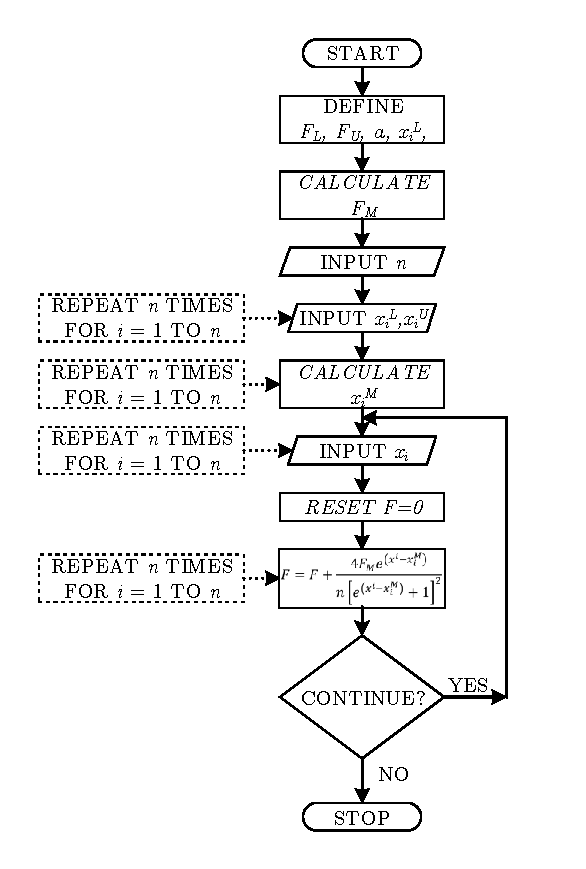
\includegraphics[width=0.48\textwidth]{images/flow-chart}
	\label{Fig:Flowchart}
	\caption{Flowchart}
\end{figure}
Figure~\ref{Fig:Flowchart} shows the proposed algorithm.
\section{Application}
\label{Sec:Application}
\section{Conclusion}
\label{Sec:Conclusion}
The mathematical construction is given in detail, which helps others to adapt to meet any additional requirements.

%\bibliographystyle{apacite}%unsrtnat}
%\bibliographystyle{spbasic}      % basic style, author-year citations
%\bibliographystyle{spmpsci}      % mathematics and physical sciences
%\bibliographystyle{spphys}       % APS-like style for physics
\bibliographystyle{ieeetr}
\bibliography{refs}
\end{document}
